\subsection{Logica de iesire}
\paragraph{}
Aceasta sectiune a documentului este dedicata implementarii blocului de afisare din Figura \ref{fig:bloc_afisare}.

\paragraph{}
Dupa cum s-a vazut la capitolul de fundamente teoretice, un controller VGA trebuie sa furnizeze cinci semnale: trei pentru culoarea curenta, si 2 pentru sincronizarea fascicolului de electroni. Din fericire, placuta \emph{Basys2} pune la dispozitie 10 semnale pe care le converteste la un port VGA dupa cum urmeaza:

\begin{figure}[h]
\centering
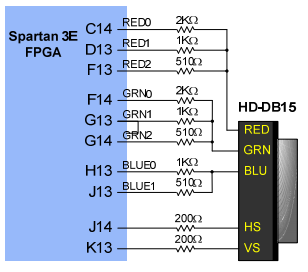
\includegraphics[width=180pt]{basys2_vga}
\caption{Basys2 VGA Port}
\label{fig:vga_pinout}
\end{figure}

Observam ca Basys2 ne pune la dispozitie trei semnale digitale pentru canalul culorii \emph{Rosu}, trei pentru \emph{Verde} si doar 2 pentru \emph{Albastru}. Impreuna formeaza un bus de 8 biti. Culoarea albastra primeste o rezolutie mai mica deoarece ochiul uman este mai sensibil la verde si rosu. Basys2 converteste aceste valori digitale la un semnal analogic pentru fiecare canal. Semnalele pentru sincronizarea orizontala si verticala sunt legate fara logica suplimentara.

\paragraph{}
Deoarece clock-ul placutei Basys2 este de {\tt50Mhz}, putem aproxima o frecventa de {\tt25.157Mhz} impartind la doi frecventa placutei. O frecventa de {\tt25Mhz} este suficienta pentru ca majoritatea monitoarelor sa se recunoasca rezolutia.

\begin{lstlisting}[frame=L]
    if rising_edge(clk) then
        if clk25MHz = '1' then
            -- logica la 25Mhz
        end if;
        clk25MHz <= not clk25MHz;
    end if;
\end{lstlisting}

\paragraph{}
Din pacate, oscilatorul placutei Basys2 nu este suficient de stabil pentru a sincroniza monitoarele moderne. Se recomanda folosirea unui oscilator separat, conectat la slotul dedicat al placutei. Autorii proiectului nu au avut acces la un oscilator stabil. Imaginea rezultata folosind oscilatorul nativ sufera de artefacte verticale. Cu toate acestea, forma de unda este vizibila si poate fi recunoscuta de catre utilizator.

\clearpage
\paragraph{}
Componenta de control a logicii de iesire are ca semnal de intrare impulsul de clock, iar ca semnale de iesire pozitia pe X si Y a fascicolului de electroni pe suprafata monitorului, impreuna cu un semnal de control care indica daca fascicolul se afla pe suprafata vizibila sau nu.

\paragraph{}
Folosind doua comparatoare, se determina daca pozitia fascicolului pe verticala ( axa Y ) se afla intre valorile esantioanelor de la adresele X, respectiv X-1. Aceasta metoda presupune ca dimensiunea memoriei de esantionare este egala cu rezolutia verticala a monitorului in pixeli, iar valorile esantioanelor sunt scalate in prealabil pentru a fi mapate direct in spatiul monitorului.

Pentru a face comparatia intre pozitia curenta si valoarea a doua esantioane intr-un singur impuls de clock ( respectiv doua, luand in considerare faptul ca fascicolul de electroni petrece doua semnale de clock deasupra unui pixel, frecventa clock-ului intern al  controllerului VGA fiind jumatate din frecventa clock-ului placutei ), se memoreaza valoarea esantionului de pe pozitia anterioara intr-un bistabil D. Daca pozitia curenta a fascicolului se afla intre valorile esantioanelor, culoarea trimisa la portul VGA este cea alba, adica \emph{"11111111"}. In caz contrar, sau daca fascicolul se afla in afara zonei vizibile, culoarea trimisa este cea neagra, respectiv \emph{"00000000"}. Acest lucru se face folosind un multiplexor legat la o logica combinationala ce foloseste valorile de iesire ale comparatoarelor, si semnalul ce indica daca fascicolul se afla in zona vizuala sau nu.

\begin{figure}[h]
\centering
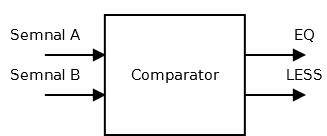
\includegraphics[width=180pt]{comparator}
\caption{Comparator}
\label{fig:comparator}
\end{figure}


Comparatoarele sunt circuite combinationale ce primesc ca semnale de intrare doua valori de comparat, si prezinta la iesire doua semnale digitale numite \emph{EQ} si \emph{LESS}, active pe '1' logic, ce au ca semnificatie:

\begin{center}
    \begin{tabular}{| l | l | l |}
    \hline
    EQ & LESS & Interpretare \\ \hline
	1 & * & Semnalele sunt egale  \\ \hline
    0 & 0 & Semnalul A este mai mic decat B  \\ \hline
    0 & 1 & Semnalul A este mai mare decat B \\ \hline 
    \end{tabular}
\end{center}

\clearpage
\begin{figure}[h]
\centering
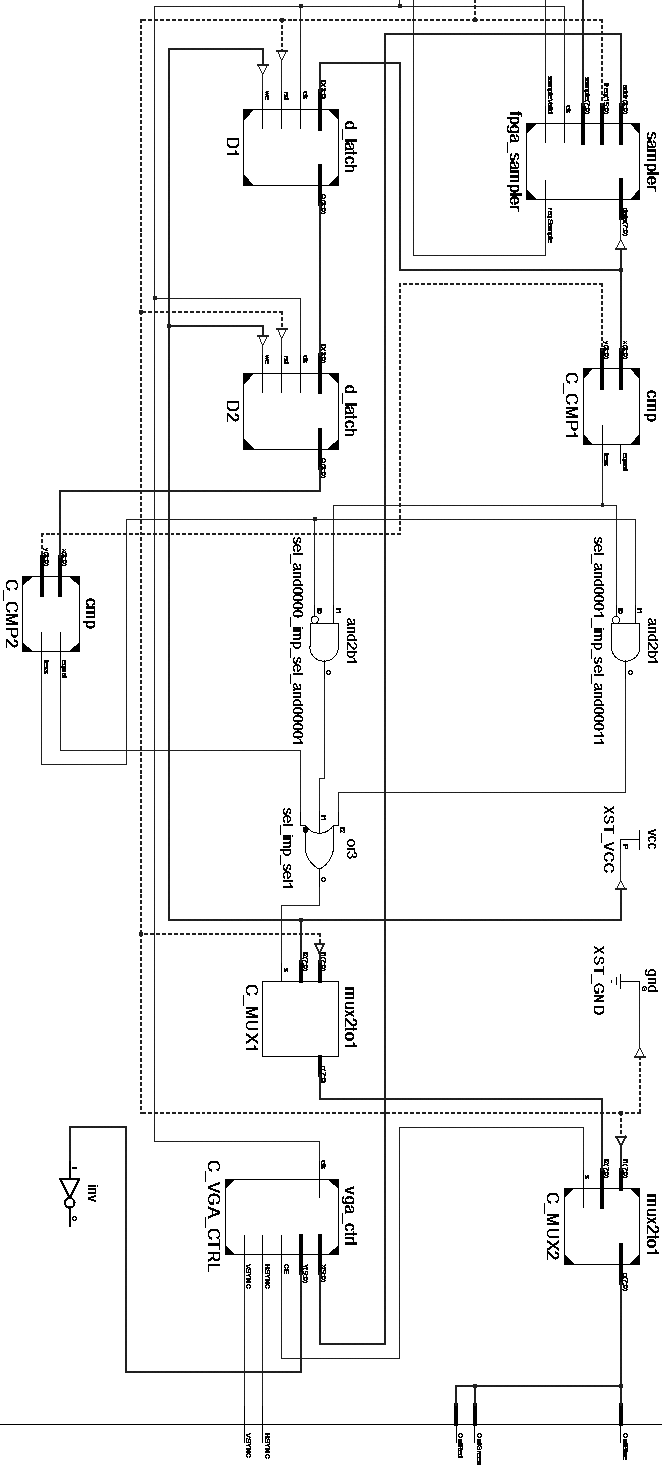
\includegraphics[width=320pt]{vga_rtl}
\caption{Schema pentru logica de iesire}
\label{fig:vga_rtl}
\end{figure}